% Created 2025-10-13 Mon 14:40
% Intended LaTeX compiler: lualatex
\documentclass[a4paper,12pt]{article}
\usepackage{amsmath}
\usepackage{fontspec}
\usepackage{graphicx}
\usepackage{longtable}
\usepackage{wrapfig}
\usepackage{rotating}
\usepackage[normalem]{ulem}
\usepackage{capt-of}
\usepackage{hyperref}
\usepackage{luacode}
\usepackage[english, french]{babel}
\usepackage{microtype}
\usepackage[autolanguage]{numprint}
\npthousandsep{~}
\usepackage{fontspec}
\usepackage{ulem}
\usepackage{soul}
\setmainfont{Source Serif 4}[Path=/home/anthea/org/fonts/Source_Serif_4/static/, UprightFont=SourceSerif4-Regular.ttf, ItalicFont=SourceSerif4-Italic.ttf, BoldFont=SourceSerif4-Bold.ttf, BoldItalicFont=SourceSerif4-BoldItalic.ttf]
\setsansfont{Source Sans 3}[Path=/home/anthea/org/fonts/Source_Sans_3/static/, UprightFont=SourceSans3-Regular.ttf, ItalicFont=SourceSans3-Italic.ttf, BoldFont=SourceSans3-Bold.ttf, BoldItalicFont=SourceSans3-BoldItalic.ttf]
\setmonofont{Source Code Pro}[Path=/home/anthea/org/fonts/Source_Code_Pro/static/, UprightFont=SourceCodePro-Regular.ttf, ItalicFont=SourceCodePro-Italic.ttf, BoldFont=SourceCodePro-Bold.ttf, BoldItalicFont=SourceCodePro-BlackItalic.ttf]
\renewcommand{\familydefault}{\sfdefault}
\renewcommand{\tiny}{\small}
\renewcommand{\scriptsize}{\small}
\usepackage[usenames,dvipsnames,svgnames,table]{xcolor}
\definecolor{customgray}{HTML}{505050}
\usepackage[top=3.2cm, bottom=3.2cm, left=2.4cm, right=2.4cm]{geometry}
\usepackage{setspace,fancyhdr,indentfirst,lastpage,datetime,authblk,ifthen,etoolbox,titling}
\singlespacing
\pagestyle{fancy}
\fancyhf{}
\fancyfoot[C]{\thepage\ / \pageref{LastPage}}
\renewcommand{\headrulewidth}{0pt}
\setlength{\parindent}{0pt}
\setcounter{secnumdepth}{3}
\setlength{\columnsep}{0.8cm}
\setlength{\marginparwidth}{1.6cm}
\setcounter{page}{1}
\usepackage{csquotes}
\usepackage{array,booktabs,multirow,tabularx,colortbl,diagbox,makecell,ltablex,adjustbox,multicol}
\usepackage{enumitem}\setlist{nosep}\setlist[itemize]{leftmargin=*}
\usepackage[toc,page]{appendix}
\usepackage[nottoc]{tocbibind}
\newenvironment{keyword}{\begin{trivlist}\item[]{\bfseries Mots-clés :}}{\end{trivlist}}
\usepackage{graphicx,caption,wrapfig}
\usepackage[most,breakable,xparse,listings,skins]{tcolorbox}
\usepackage[colorinlistoftodos]{todonotes}
\usepackage{newfloat}
\DeclareFloatingEnvironment[fileext=lol,listname={\vspace{-2em}},name=Listing]{listing}
\captionsetup{format=plain,font=small,labelfont=bf}
\captionsetup[listing]{labelfont=bf,textfont=it}
\usepackage{fvextra,amsfonts,amssymb,amsmath,mathrsfs,mathtools,stmaryrd}
\usepackage{algorithm2e}
\usepackage{pgf,tikz,pgfplots,pgfplotstable,arydshln,subcaption,forest}
\pgfplotsset{compat=1.18}
\usepackage[acronym]{glossaries}
\makenoidxglossaries
\usepackage{url,orcidlink,hyperref}
\hypersetup{colorlinks=true, linkcolor=customgray, citecolor=customgray, urlcolor=customgray, pdfborder={0 0 0}, unicode=true}
\author{Cyprien Pierre1,2, Alexis Heloir1 , and Christophe Kolski1}
\date{\today}
\title{L’ingénierie de la construction, un environnement multi-contraint : constat et perspectives}
\hypersetup{
 pdfauthor={Cyprien Pierre1,2, Alexis Heloir1 , and Christophe Kolski1},
 pdftitle={L’ingénierie de la construction, un environnement multi-contraint : constat et perspectives},
 pdfkeywords={},
 pdfsubject={},
 pdfcreator={},
 pdflang={French}}
\usepackage[style=backend=biber,style=iso-numeric,citestyle=numeric-comp,doi=true,isbn=true,mincrossrefs=2,autocite=superscript]{biblatex}
\addbibresource{~/org/references.bib}
\begin{document}

\maketitle
1 LAMIH UMR CNRS 8201, Université Polytechnique Hauts-de-France, 59301 Valenciennes Cedex, France
2 EIFFAGE ENERGIE SYSTEMES, 40 rue du Bignon 35135 Chantepie, France
\begin{otherlanguage}{english}
\begin{abstract}
Construction projects are increasing in complexity, as are customers’ needs. Meanwhile, legislation tightens, and standards proliferate. Projects turned into over-constrained problems. A constraint is any part of a requirement that the contractor and its partner organizations should satisfy. This research project aims to design, implement, and assess a constraint-focused environment capable of improving compliance reporting in construction engineering with a specific focus on electrical engineering. Three aspects structure the project: automated dynamic extraction of functional and organizational constraints, innovative human-machine interaction supporting the reporting and resolution of unsatisfied constraints, and adaptation of agile methodologies commonly used in software engineering to improve collaboration in Building Information Modeling
 (\protect\hyperlink{gls-1}{\label{gls-1-use-1}BIM}) projects.
\end{abstract}

\begin{keyword}
Keywords. Human-machine interaction, Constraint sensitivity, Compliance, Project approach, Electrical engineering.
\end{keyword}
\end{otherlanguage}

\begin{abstract}
Les projets de construction se complexifient. Les besoins des clients augmentent, la législation se durcit et les normes prolifèrent. Les projets sont devenus des environnements sur-contraints. Une contrainte est tout élément d’exigence devant être respecté par le système de construction et par les organisations partenaires. Ce projet de recherche vise à concevoir, réaliser et évaluer une interface utilisateur sensible aux contraintes pour améliorer la remontée de conformité en ingénierie de la construction. Nous nous concentrons sur l’électrotechnique. Le projet s'articule autour de trois axes principaux : l'extraction dynamique des contraintes fonctionnelles et organisationnelles par une approche algorithmique, l'amélioration de l'interaction humain-machine permettant la remontée et la résolution des contraintes non satisfaites et l'adoption de méthodologies agiles inspirées du génie logiciel en vue d’améliorer l’intégration des démarches de projet \protect\hyperlink{gls-1}{\label{gls-1-use-2}BIM}. 
\end{abstract}

\begin{keyword}
Interaction humain-machine, Sensibilité aux contraintes, Conformité, Démarche de projet, Electrotechnique.
\end{keyword}
\section{Introduction}
\label{sec:orgcdcc8a9}
L’industrie de la construction connaît une transformation profonde depuis les années 2000 avec l’émergence des outils de \protect\hyperlink{gls-1}{\label{gls-1-use-3}BIM} et d’aide à la décision. L’augmentation des capacités de calcul permet de réaliser des simulations des systèmes de construction de plus en plus précises et complexes. L’informatique en nuage  offre un cadre technique propice à la collaboration en temps réel. Pour autant, la filière se confronte toujours à des contraintes émanant de différents corps de métiers et acteurs, dans les démarches de projets. Nous tentons d’en simplifier les appréciations et résolutions par une approche d’interaction humain-machine. Cette recherche s’inscrit dans le cadre d’une thèse CIFRE démarrée en 2025. Une contrainte se définit ici comme une exigence formalisée (réglementaire, normative ou spécifique à un projet) qu’un système de construction et les parties prenantes doivent satisfaire. Comme exprimé dans la norme ISO 19650-1 \autocite{OrganisationNumerisationInformations2018a}, il s’agit d’une information de contexte permettant la compréhension des études réalisées.  Une question de recherche importante dans le cadre de nos travaux peut être résumée de la manière suivante : comment rendre les contraintes compréhensibles, exploitables, interactives et collectivement négociables pour les acteurs concernés ?

Au sujet des contraintes, le \protect\hyperlink{gls-1}{\label{gls-1-use-4}BIM} propose une approche de l'ingénierie partagée et dont l’intention du client \footnote{Le client est la personne physique ou morale finançant le projet de construction.} est préservée sur l’ensemble du processus. Les technologies du \protect\hyperlink{gls-1}{\label{gls-1-use-5}BIM} permettent de modéliser les composants d'un bâtiment et d'en vérifier les contraintes de matériaux, de géométrie et d’apparence. Des outils collaboratifs dédiés ont accompagné le développement et l’adoption de la méthodologie et des standards du \protect\hyperlink{gls-1}{\label{gls-1-use-6}BIM}, outils accompagnés de leur cortège de contraintes spécifiques aux besoins de la collaboration entre les structures de décision, les pratiques et les métiers historiques. 

Les principes généraux du \protect\hyperlink{gls-1}{\label{gls-1-use-7}BIM} reposent sur un schéma organisationnel existant dans l’industrie manufacturière depuis les années 1960 \autocite{caelenConsommateurAuCoeur2004a} : l' Integrated Concurrent Engineering
 (\protect\hyperlink{gls-2}{\label{gls-2-use-1}ICE}) \autocite{delsavioVirtualDesignConstruction2022}. La transposition de l’\protect\hyperlink{gls-2}{\label{gls-2-use-2}ICE} à l’industrie de la construction se confronte à des difficultés systémiques de mise à l’échelle. L’approche Virtual Design and Construction
 (\protect\hyperlink{gls-3}{\label{gls-3-use-1}VDC}) unifie les approches du \protect\hyperlink{gls-1}{\label{gls-1-use-8}BIM} et de l’\protect\hyperlink{gls-2}{\label{gls-2-use-3}ICE}. Un des cas d’usage du \protect\hyperlink{gls-3}{\label{gls-3-use-2}VDC} est  l’implication des exploitants \footnote{L’exploitant est la personne physique ou morale bénéficiant de l’actif construit.} dans la précision des contraintes \autocite{delsavioVirtualDesignConstruction2022,mathiaspettergustafssonRoleVDCProfessionals2015a}. Les environnements collaboratifs associés au \protect\hyperlink{gls-3}{\label{gls-3-use-3}VDC} permettent une meilleure appréciation des contraintes temporelles de mise en œuvre des bâtiments. Des études récentes soutiennent que l'adoption du \protect\hyperlink{gls-3}{\label{gls-3-use-4}VDC} facilite la coopération entre les acteurs de la construction \autocite{delsavioVirtualDesignConstruction2022,mugheesaslamIntegratedImplementationVirtual2021}. Cependant, l'adoption généralisée est toujours entravée par des contraintes organisationnelles.

L’observation se poursuit avec l’émergence des Building Information System
 (\protect\hyperlink{gls-4}{\label{gls-4-use-1}BIS}) et la création de Building Operating System
 (\protect\hyperlink{gls-5}{\label{gls-5-use-1}BOS}). Le \protect\hyperlink{gls-4}{\label{gls-4-use-2}BIS} et le \protect\hyperlink{gls-5}{\label{gls-5-use-2}BOS} imposent un cadre de conception qui inclut les utilisateurs \footnote{L’utilisateur est toute personne physique interagissant avec l’actif construit.}. L’étendue du champ d’application de cette thématique semble forcer l’émergence d’un lot Informatique aux côtés des lots historiques de la construction \autocites{mohamedyassinebenjemaaImplementationSolutionsIntegrees2017a}[][]{cottetSystemesTempsReel2005}{smartbuildingallianceBISBOSOutils2022}. Cette mutation entraîne la nécessité de respecter un nouvel ensemble de contraintes lié à l’informatique et à sa sécurité.

L’apport de technologies numériques n’est pas l’unique vecteur de transformation du secteur. Un second se distille par la régulation des pratiques et des volontés d'homogénéité concourant à l’élaboration d’un environnement fortement contraint \autocite{benzerafa-alilatLinflationNormativeLamplification2022a}. Ces contraintes sont formalisées par des institutions externes \autocite{artokiviniemiPREMISSRequirementsManagement2004} à travers notamment le cadre législatif et normatif. L’adoption des standards et des bonnes pratiques liées au \protect\hyperlink{gls-1}{\label{gls-1-use-9}BIM} comme au \protect\hyperlink{gls-3}{\label{gls-3-use-5}VDC} devait permettre d’augmenter l’efficacité lors des phases de conception et d’optimiser les phases d’exécution des projets de construction. Ces bénéfices sont acquis au prix d’une augmentation des contraintes à considérer durant les cycles d’études \autocite{shahruddinBIMRequirementsConstruction2020a}. 

Cet environnement sur-contraint pose un obstacle à la collaboration et la prise de décision \autocite{adriennecostaConstructionNormeLarchitecte2012}. Il convient alors d'examiner l'état des connaissances et des pratiques existantes pour identifier les redondances et les divergences entre  les contraintes métiers pour proposer un cadre unifié et structuré capable de factoriser et hiérarchiser ces contraintes. Une attention particulière sera portée à la conception de systèmes électriques, domaine de prédilection du partenaire industriel de ce travail de recherche.

Dans la suite de cet article, nous décrivons l’état de l’art relatif à la gestion du cycle de vie des contraintes dans le domaine de la construction. Nous réalisons ensuite une analyse contextualisée en électrotechnique. De ces prémisses, nous définissons nos axes de recherche en vue de répondre à notre question préliminaire. Ce cadre s’accompagne des perspectives de travaux à mener pour valider nos intentions. À l'issue de la conclusion, nous terminons par un propos prospectif sur la poursuite de nos études.
\section{Etat de l’art}
\label{sec:org91d9d7b}
\subsection{Cycle de vie des contraintes de construction}
\label{sec:orge9f62f3}
Le recensement des contraintes est l’une des étapes les plus importantes d’un projet et dont les erreurs occasionnent d’irrémédiables impacts \autocite{mabeloRequirementsManagementProject2025a}. La multiplicité des sources de contrainte complexifie le processus de collecte et implique d’analyser des sources multiples et diverses : 
\begin{itemize}
\item réglementaires, issues des textes de loi et expriment des contraintes de nature organisationnelle et ayants trait aux aspects économiques, administratifs et sociaux \autocite{devinazRapportDinformationFait2023}, dont la rédaction se conforme au Guide de légistique \autocite{GuideLegistique2017a} en France,
\item normatives, issues de travaux pilotés par des agences d’Etat et dont la rédaction suit le Guide 59 \autocite{PratiquesNormalisationRecommandees2019a} pour l’ISO,
\item standardisées, issues de recueils de bonne pratiques ou de référentiels harmonisés portés par un ou plusieurs acteurs de l’industrie et ayant fait consensus,
\item contextuelles, issues des spécifications propres à un projet (cahier des charges, spécifications techniques, contrat de prestation\ldots{}) sans standards formels de rédaction.
\end{itemize}

Les deux premières sources représentent la majeure partie du corpus de contraintes dont il est estimé que 90\% proviennent des réglementations et 10\% des normes \autocite{baudetTropNormesAFNOR2024}. La nature des contraintes exprimées par des sources contextuelles est de tendance évolutive, pouvant être modifiée régulièrement durant le cycle de conception et de construction d’un actif.

Chaque contrainte identifiée est reliée via une table de correspondance à des documents de projet qui décrivent la manière dont la contrainte a été prise en compte. Cet aspect d’un projet de construction est porteur d’un risque significatif d'erreurs d'interprétations ou d'oublis,  risque amplifié par le manque d'ergonomie et le manque d'efficience dans la gestion, la présentation et la contextualisation des sources. En outre, certains textes expriment parfois des contraintes contradictoires, ce qui augmente les risques de retards liés à la nécessité d’obtenir un consensus de la part d’acteurs dont les intérêts peuvent diverger  à défaut de règles d’arbitrages \autocite{EntryForceEuropean2024a,robertorodriguezCoherenceOuContradiction2022}.

Les documents sont organisés dans un système de Gestion Electronique des Documents
 (\protect\hyperlink{gls-6}{\label{gls-6-use-1}GED}) \autocite{pimoMisePlaceSolutions2021a}. Une \protect\hyperlink{gls-6}{\label{gls-6-use-2}GED} associe des  métadonnées aux fichiers et automatise les processus auxquels les documents sont intégrés. La configuration des \protect\hyperlink{gls-6}{\label{gls-6-use-3}GED} en ingénierie de la construction est une opération lourde et complexe, réalisée par un spécialiste au début de chaque projet \autocite{bjorkElectronicDocumentManagement2006a}. Une \protect\hyperlink{gls-6}{\label{gls-6-use-4}GED}  automatise la gestion du cycle de vie des documents (signatures, diffusion, archivage, etc.). Si une \protect\hyperlink{gls-6}{\label{gls-6-use-5}GED} peut être complétée par des correcteurs orthographiques et des systèmes de mise en page automatiques, il n'existe pas de solution permettant de valider son contenu.

En parallèle, un ensemble d’acteurs prépare des listes d’informations associées aux maquettes numériques et identifiées comme nécessaires au bon déroulement du projet. Ces besoins sont compilés dans un fichier standardisé appelé Information Delivery Specifications
 (\protect\hyperlink{gls-7}{\label{gls-7-use-1}IDS}) \autocite{InformationDeliverySpecification2024a}. Ce fichier permet de réaliser des opérations de vérification automatique de qualité des données (présence d’un attribut, existence d’une valeur, respect d’une unité…).

Après ces étapes de modélisation, un ou plusieurs référents sont identifiés pour assurer le suivi de la prise en compte des contraintes. Ce suivi souffre d'un caractère non-exécutable, impliquant une exploration systématique par les référents  des corpus documentaires lors des étapes de vérification et de contrôle.

Les contraintes peuvent être classées selon trois natures :
\begin{itemize}
\item technique : contraintes liées au respect de conditions et de règles d'un métier donné,
\item fonctionnelle : contraintes liées à la réponse à un besoin de fonctionnement d'une installation,
\item organisationnelle : contraintes de toutes autres natures.
\end{itemize}

Des protocoles et procédures sont mis en œuvre pour assurer la satisfaction de ces contraintes. La figure \ref{fig:org0a4a908} présente le cycle de vie des contraintes dans un projet de construction.


\begin{figure}[htbp]
\centering
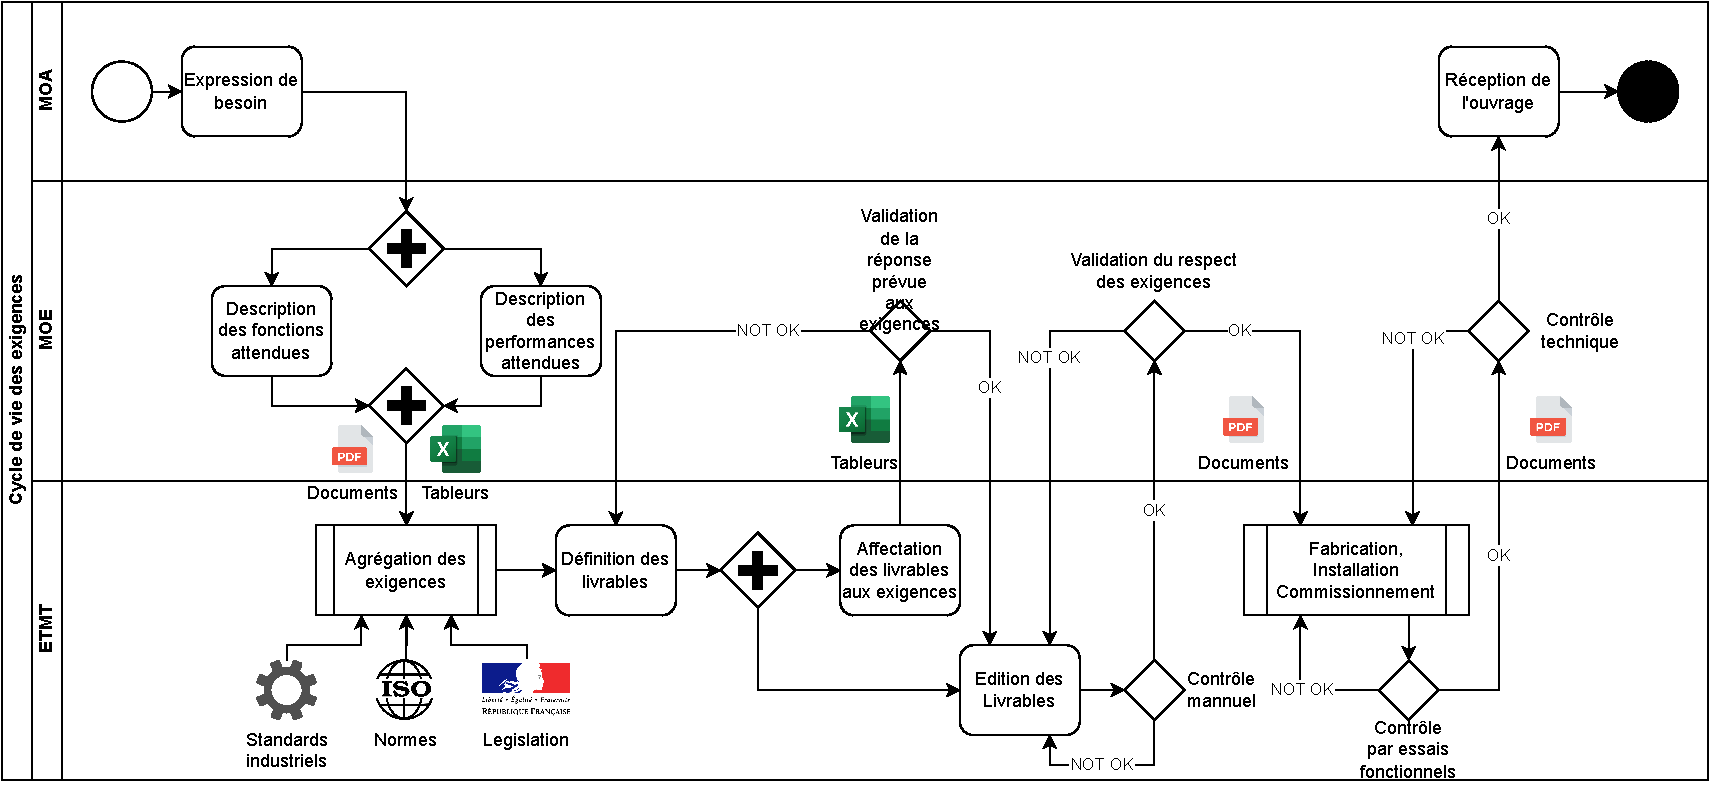
\includegraphics[width=.9\linewidth]{../svg/BPMN-LifeCycle-Exigences-init.pdf}
\caption{\label{fig:org0a4a908}Macro-processus de traitement des contraintes durant un projet de construction.}
\end{figure}

Comme visible en Figure \ref{fig:org0a4a908}, la Maitrise d’OuvrAge
 (\protect\hyperlink{gls-8}{\label{gls-8-use-1}MOA}) définit les besoins. Ceux-ci sont précisés par la Maitrise d'Œuvre
 (\protect\hyperlink{gls-9}{\label{gls-9-use-1}MOE}) puis intégrés par l' Entreprise Titulaire d'un Marché de Travaux
 (\protect\hyperlink{gls-10}{\label{gls-10-use-1}ETMT}). Cette dernière est alors responsable de la supervision des contraintes, des moyens d’y répondre, de la réalisation des études et de l'exécution des travaux. Les deux acteurs précédents assurent des rôles d'approbation ou de support. On constate qu’on impose généralement au dernier acteur d’un cycle de conception le respect d’un corpus de contraintes dont il n’a pas participé à l’élaboration. Par ce fonctionnement, l’ensemble des responsabilités semble concentré sur le constructeur.

Les outils informatiques actuels permettent de répondre convenablement aux contraintes techniques. La modélisation procédurale permet de générer des modèles numériques respectant un ensemble de contraintes géospatiales et géométriques \autocite{s.dineshkumarBIMbasedAutomatedSite2015}. La réalisation de notes de calculs, les simulations et les mesures physiques sont des moyens complémentaires permettant de prouver l’atteinte d’un objectif technique \autocite{tomc.borstBIMSimulation2015,galSimulationEnergetiqueDynamique2025a}. Ces aspects sont tout de même chronophages, car ils nécessitent des étapes de configuration et de paramétrage, comparés aux solutions nouvelles employant des modèles génératifs \autocite{chaillouLintelligenceArtificielleAu2021a}. Les configurations sont réalisées généralement par des experts et la vérification des rapports extraits des simulations demande également un haut niveau de technicité \autocite{delsavioVirtualDesignConstruction2022}. Le plus souvent, les outils sont utilisés en silos et ne permettent pas de partager un environnement de contraintes commun \autocite{moreauConceptionElectriqueQuelles2019a}. Les itérations permettant d’aboutir à une solution viable pour un aspect métier (électrotechnique, mécanique, etc.) peuvent entraîner la mise en défaut de contraintes d’un autre aspect métier \autocite{vandebrugInterdisciplinaryConfigurationMethods2025a}. Il serait intéressant d’établir un cadre d'exécution des vérifications des contraintes partagé pour favoriser l’abandon rapide des itérations aux solutions parasitantes.

Actuellement, il n'existe pas de système permettant d’assurer le respect des contraintes fonctionnelles et organisationnelles à un niveau qualitatif équivalent à ceux destinés aux contraintes techniques. Ce périmètre est alors limité à l'apport en connaissances individuelles et repose entièrement sur un système de confiance pair-à-pair. Ce système de confiance, couplé au cloisonnement des compétences, crée un environnement de doute contraignant les processus d'acceptation en multipliant les contraintes d’approbation. On peut toutefois mentionner l’existence de recherches relatives à la mise en œuvre de protocoles de validation permettant de soulager la charge de la preuve et du manque de confiance entre les parties au moyen de technologies de cryptographie et de chaîne de blocs \autocite{mathewsBIM+BlockchainSolutionTrust2017a}. 
\subsection{Focus sur l’électrotechnique et ses contraintes}
\label{sec:org7b7a302}
Les bâtiments contemporains sont parcourus par de nombreux réseaux électriques de différentes natures : signalisation, données, puissance. La diversité de ces réseaux implique une gestion complexe de contraintes diverses et sophistiquées : il peut s'agir d'interface avec le génie climatique sur l'alimentation d'équipements et des remontées de capteurs, de mise en oeuvre de systèmes complexes de détection d'incendies reliés avec les sapeurs pompiers locaux ou encore la réalisation d'un réseau de surveillance et de sécurité assujetti à des dispositions de résilience informatique. La multiplicité des domaines techniques appliqués à la gestion des réseaux électriques augmente la quantité de clauses contractuelles ainsi que le corpus normatif et législatif à prendre en responsabilité par les entreprises. 

Lors de la réalisation des études électrotechniques chez Eiffage Energies Systèmes (EES), les opérations sont découpées au regard des compétences nécessaires à leur aboutissement. Ainsi, un pôle spécialisé en distribution de courant s’occupe de notes de calculs et de schématiques, un autre se spécialise dans les études de conversion de fréquences, une équipe code les programmes d’automatisme, un collaborateur intègre les composants d’automatisme dans les schémas électriques préalablement préparés par le premier pôle présenté, un coordonnateur collecte et met en cohérence les besoins en matières de câbles, un autre pilote l’attribution de code d’identification, un pôle modélise les installations en 3D, certains de ses membres ont une spécialité en mécanique, en électromécanique ou encore en préparation de chantier. 

En zoomant sur cette organisation, nous observons une grande diversité de compétences associées à des référentiels spécifiques. Elles s’étendent par exemple de la mise en oeuvre des normes de sécurité incendie, de l’Eurocode 3 \autocite{icabEurocodesCodesConstructiona} sur la fixation des éléments jusqu’aux habilitations Qualifoudre \autocite{charpentierReferentielPourCertificationa}. Ces éléments sont rarement maîtrisés simultanément. L’empilement des référentiels techniques à respecter entraîne des contraintes en matière de gestion des ressources humaines des projets.

La diversité des équipes permet à l’entreprise de réaliser un large périmètre d’étude sans recourir à des sous-traitants. Cependant, le maintien des compétences en interne associé à leur haute concentration entraîne un risque de perte de compétences en cas d’imprévu. Ce problème implique également des difficultés de vérification interne des études produits lorsqu’une thématique n’est maîtrisée que par une ou deux personnes.

Chaque sous-domaine requiert généralement l’approbation d'un expert intervenant souvent en fin de cycle de conception. Cette intervention peut arriver trop tardivement : une infraction de contrainte critique peut nécessiter le renvoi du projet en amont de la phase de conception et entraîner des surcoûts et des retards. À titre d’exemple, sur un projet d’électrification d’un bassin de maintenance d’un navire, des imprécisions dans les étapes de conception ont conduit à une sous-estimation des besoins en dimensions et en nombre de câbles. Cela a engendré des complexités supplémentaires pour EES lors de la réalisation de son marché de travaux. L’entreprise d’électricité, dès son intégration au projet, a réétudié le dimensionnement des besoins de câbles de façon précise et a fait observer que les caniveaux spécifiés étaient plus de deux fois trop petits pour permettre l’accueil des besoins réels en canalisations électriques. Cette erreur a nécessité le renvoi du projet en bureau d’études pour identifier de nouveaux cheminements et modes de pose.

Un tel enchaînement d'événements pourrait être évité en proposant aux acteurs de la phase de conception des outils interactifs et intuitifs permettant d’éviter en amont les infractions aux contraintes électriques. Il s'agirait de rendre explicites le fonctionnement et les contraintes des différents flux électriques, leurs interférences avec les équipements environnants ainsi que les autres réseaux,leurs contraintes sécuritaires et normatives par des retours visuels et textuels adaptés. Dans ce but, il est important de respecter les critères d'utilisabilité au sens de la norme ISO 9241-11:2018 \autocite{ErgonomieLinteractionHommesysteme2018}, et de vérifier la cohérence avec la démarche cognitive inhérente à la phase de conception, pour chaque acteur concerné. Il serait ainsi possible de garantir le respect de ces contraintes à chaque modification du projet ou à intervalles réguliers à la manière des tests unitaires dont la pratique a été systématisée dans l'industrie du génie logiciel.

La complexification croissante des bâtiments, notamment due à leur informatisation \autocite{DecretNdeg20208872020,SmartReadinessIndicatora}, crée de nouveaux besoins impliquant de nouvelles compétences. Ainsi, sur des projets d’envergure, la multiplicité des besoins en systèmes informatiques est telle qu’il devient nécessaire de composer des équipes d'experts pour en assurer le suivi. Il existe historiquement les systèmes de Gestion Technique du Bâtiment
 (\protect\hyperlink{gls-11}{\label{gls-11-use-1}GTB}), de Gestion Technique Centralisée
 (\protect\hyperlink{gls-12}{\label{gls-12-use-1}GTC}), de sécurité incendie, de Voix, Données et Images
 (\protect\hyperlink{gls-13}{\label{gls-13-use-1}VDI}) et les Système de Contrôle et d'Acquisition de Données
 (\protect\hyperlink{gls-14}{\label{gls-14-use-1}SCADA}). Ceux-ci sont désormais complétés par des systèmes de réseaux IP privés tels que les réseaux Multiprotocol Label Switching
 (\protect\hyperlink{gls-15}{\label{gls-15-use-1}MPLS}), de diffusion de réseaux 5G privés et de divers systèmes d’Internet of Things
 (\protect\hyperlink{gls-16}{\label{gls-16-use-1}IoT}). Ces nouveaux éléments ajoutent des contraintes conséquentes liées aux infrastructures informatiques et à la sécurisation des services.

Lors de la phase d’organisation d’un marché global de performance portant sur la création d’un technicentre, EES a rassemblé une équipe dédiée à la prise en charge du périmètre des technologies de l’information. Elle est missionnée dans la gestion des risques de cybersécurité, l'ingénierie des réseaux informatiques, la conception de centres de données, la mise en œuvre d’environnements de travail virtualisés, dans l’intégration des services applicatifs et pilote les opérations de collecte et d’analyse de données. L’entreprise observe que ces thématiques représentent collectivement un volet important sur le projet mentionné, rivalisant avec les lotissements habituels. 

L'analyse des méthodes actuelles de traitement des contraintes révèle des lacunes significatives, particulièrement en ce qui concerne les contraintes fonctionnelles et organisationnelles. Ces limitations se manifestent avec une acuité particulière dans le domaine de l'électrotechnique, où la complexité croissante des systèmes et la multiplicité des intervenants amplifient les difficultés de coordination et de vérification de conformité. Les défis identifiés illustrent parfaitement les verrous systémiques qui entravent l'efficience des processus de conception et de construction. Face à ces constats, il devient nécessaire de définir des orientations de recherche susceptibles de proposer des solutions pour automatiser et optimiser la gestion des contraintes dans ce secteur spécialisé.
\section{Axes de recherche}
\label{sec:orgdfcf293}
Cette recherche vise à proposer des pistes permettant de lever les verrous qui freinent l'exécution efficiente de la remontée de conformité en ingénierie de systèmes électriques. Une remontée de conformité est une réponse qualitative à une contrainte. Elle s’inscrit dans un cadre de réponse aux enjeux génériques des entreprises de construction tels que le management de la qualité, la gestion des risques, la maîtrise des coûts, la maîtrise des délais et la capitalisation sur l’expérience \autocite{ManagementProjetProgramme2017}.

Différentes solutions de l'état de l’art seront étudiées afin de permettre l’extraction dynamique des contraintes fonctionnelles et organisationnelles. Les solutions étudiées seront tirées des domaines de traitement des langues naturelles appliqués aux corpus de textes réglementaires et législatifs ainsi que de l'état de l’art dans le domaine de la création et de l’échange d’ontologie appliquées au \protect\hyperlink{gls-1}{\label{gls-1-use-10}BIM}. D’autres approches seront étudiées telles que les approches déclaratives, reposant sur des langages textuels ou visuels, combinées à des systèmes de gestion des règles métiers.

Lorsqu’une contrainte est enfreinte, il est nécessaire de remonter à l'utilisateur non spécialiste la nature de l’infraction, sa ou ses causes et une ou plusieurs suggestions capables de lever l’infraction observée. Les solutions étudiées porteront sur les travaux liés à la conception d’Interfaces Utilisateur (UI) \autocite{Shneiderman2016}, la prise en compte de critères de l’eXpérience Utilisateur (UX) \autocite{Nogier2020} et la réduction de la charge mentale de travail \autocite{longoHumanMentalWorkload2022a,morayMentalWorkloadIts1979a} en situation d’interaction humain-machine. 

Parmi les approches étudiées, celle dite d'interface écologique fera l’objet d’une attention particulière \autocite{Burns2004,vicenteEcologicalInterfaceDesign1992b}. Le but de telles interfaces est de rendre perceptivement évidentes à l'utilisateur les contraintes et les relations complexes constitutives de l’environnement de travail. L’approche sensible au contexte \autocite{deyUnderstandingUsingContext2001a} sera également étudiée.

Les outils ne sont pas neutres \autocite{borremansGuideConvivialTools1979a}. Ils permettent d’accompagner l’adoption de nouvelles méthodologies de travail. Les méthodes étudiées porteront notamment sur les pratiques agiles adoptées par l’industrie du génie logiciel et sur leur mise en place éventuelle dans le domaine de la construction. Nous étudierons en particulier comment la gestion itérative des modifications successives au projet (versioning) peut influencer l’organisation de la collaboration entre les différents acteurs d’un projet de construction.

Le processus présenté en figure \ref{fig:org0a4a908} pourra évoluer vers une version allégée dont la figure \ref{fig:org8957f45} propose un exemple.

\begin{figure}[htbp]
\centering
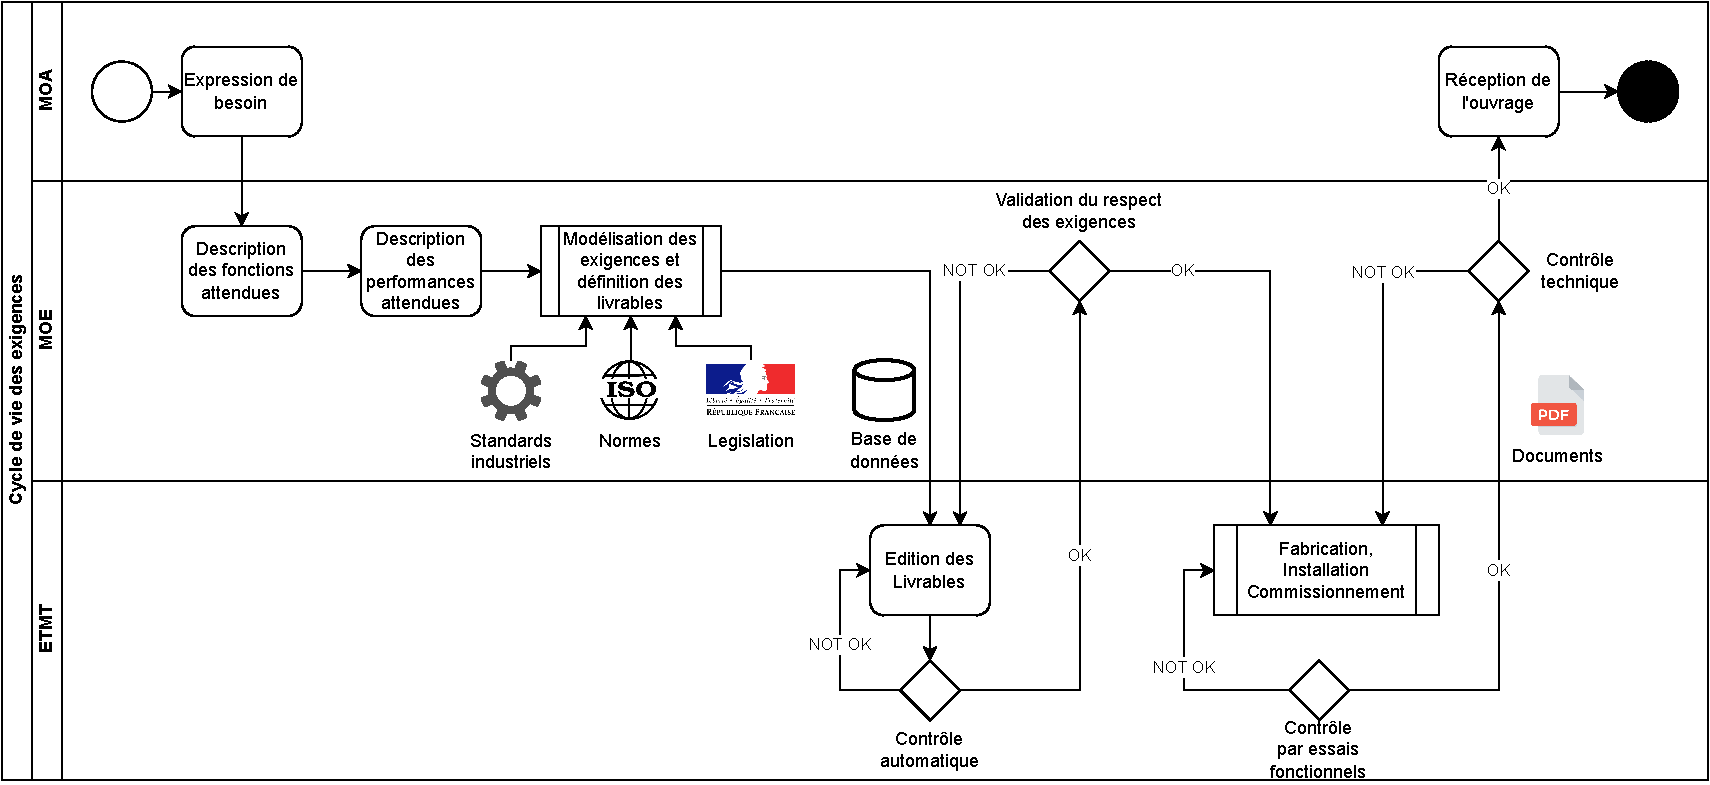
\includegraphics[width=.9\linewidth]{../svg/BPMN-LifeCycle-Exigences-target.pdf}
\caption{\label{fig:org8957f45}Macro-processus de traitement des contraintes durant un projet de construction avec automatisation des vérifications d’études.}
\end{figure}

L’évolution de ce processus devrait permettre de répartir objectivement les responsabilités des trois catégories d’acteurs : 
\begin{itemize}
\item La \protect\hyperlink{gls-8}{\label{gls-8-use-2}MOA} définit les besoins. Elle valide la réponse à ses besoins et reçoit l’ouvrage construit.
\item La \protect\hyperlink{gls-9}{\label{gls-9-use-2}MOE} transforme les besoins en un corpus de contraintes. Elle est responsable du respect de ces contraintes.
\item L’\protect\hyperlink{gls-10}{\label{gls-10-use-2}ETMT} explore l’espace de solution pour produire des études respectant les contraintes. Celles-ci validées, elle met en œuvre ses études. Elle est responsable du parfait achèvement des constructions.
\end{itemize}

Trois volets de recherche sont considérés : un volet d’ordre applicatif, un volet lié à l'interaction humain-machine, un volet d’ordre méthodologique. La définition de ces trois volets de recherche établit le cadre théorique et conceptuel nécessaire à l'élaboration d'une approche intégrée. Cette démarche trouve sa concrétisation dans la mise en œuvre d'une étude de cas spécifique qui permettra de valider les hypothèses formulées et de tester les solutions envisagées, selon les perspectives décrites ci-après.
\section{Perspectives des travaux}
\label{sec:orgb3244b7}
Notre étude des systèmes de contraintes sera guidée et illustrée par l’analyse d’un poste électrique haute tension et basse tension destiné à l'alimentation de systèmes ferroviaires. 

Ce type de construction répond à trois besoins pour notre sujet : 
\begin{itemize}
\item un périmètre restreint limitant le nombre de contraintes,
\item un sujet réel circonscrit à un petit bâtiment,
\item une construction impliquant différentes catégories d’acteurs.
\end{itemize}

La conception de postes de transformation étant un sujet maîtrisé chez notre partenaire industriel, cette étude nous permettra de confronter nos résultats à des cas d’études réels. 

Construire un poste de transformation implique la collaboration du génie civil, du génie climatique et fluidique ainsi que du génie électrique. Ce sujet offre également la possibilité d’explorer les modalités de fabrication hors site, de gestion de la sous-traitance et de gestion de la chaîne logistique qui en découle ainsi que des contraintes liées à la sécurité des personnes ou au maintien en condition opérationnelle. L’intégration de postes transformateurs soulève également des sujets d'innovation avec les mises en réseau intelligentes et de cybersécurité industrielle \autocite{flausCybersecuriteInstallationsIndustrielles2018a}.

Pour mettre à l’épreuve notre sujet de recherche, nous concevrons un démonstrateur permettant aux ingénieurs d’apprécier les systèmes de contraintes inhérents à la conception de systèmes électriques. Il sera composé d’une interface graphique adaptative permettant l’abstraction des contraintes, leur manipulation et l’identification de leurs interactions (hiérarchies, prévalence, incompatibilités, etc.). À cette interface, sera associé un système de création de contraintes ainsi qu’un système d’évaluation des contraintes. Enfin, un mécanisme de vérification devra permettre de valider le respect des contraintes établies sur un modèle numérique du cas d’étude. A ce sujet, un modèle numérique est un ensemble de fichiers de toute nature et contenant les informations générées par l’ensemble des acteurs d’un projet \autocite{OrganisationNumerisationInformations2018a}. Il conviendra donc de préciser la nature des fichiers adaptés à l'exécution des vérifications.

En parallèle, l’organisation des projets doit évoluer pour intégrer une nouvelle méthodologie et réorganiser le partage des contraintes. Pour cela, nous favorisons l’identification d’un lot informatique exerçant de concert avec les lotissements traditionnels des projets de construction. L’équipe constituante sera chargée de sélectionner, configurer, fiabiliser et maintenir le Common Data Environment
 (\protect\hyperlink{gls-17}{\label{gls-17-use-1}CDE}). La configuration inclut l’enrichissement des contraintes, des procédures et des automatisations. L’équipe sera également responsable de la planification du reste du cycle de vie de cet environnement de données : sa transformation pour supporter les opérations de travaux puis les opérations de commissionnement permettant le transfert de données au \protect\hyperlink{gls-4}{\label{gls-4-use-3}BIS} du nouveau bâtiment. 

Le lot informatique aura également la responsabilité des études de conception, de réalisation et de maintenance du \protect\hyperlink{gls-4}{\label{gls-4-use-4}BIS}. En cette qualité, il possèdera les pouvoirs nécessaires pour orienter et coordonner les choix technologiques (interfaces de programmation, protocoles de communication…) intégrés par d’autres lotissements (électrotechnique, génie climatique…). Enfin, cette organisation s’attachera à définir et préparer les applicatifs nécessaires à la vie à venir du bâtiment en matière de gestion, occupation, exploitation et maintenance. 

Un protocole expérimental sera mis en œuvre pour valider les résultats du démonstrateur dans un environnement collaboratif contrôlé (en laboratoire) puis dans un environnement réel de production.
\section{Conclusion}
\label{sec:orgbbd3605}
Face à la complexification du secteur de la construction, marquée par l'intégration des outils numériques et une inflation réglementaire, la gestion des contraintes est devenue un enjeu majeur. Les méthodes actuelles de traitement des contraintes, particulièrement pour les aspects fonctionnels et organisationnels, présentent des lacunes importantes qui entravent l'efficience des processus de conception, notamment dans le domaine de l'électrotechnique.
Cette recherche vise à contribuer à l’exploration des espaces de solutions en électrotechnique. Le développement d’une méthode d’ingénierie par contraintes devrait permettre de réduire la charge mentale des acteurs de la construction en déléguant aux solutions informatiques la responsabilité de la vérification. Une telle avancée pourrait ainsi diminuer les besoins en ressources humaines pour ces opérations et favoriser la redéfinition de missions à plus forte valeur ajoutée pour les collaborateurs.
La conduite de nos travaux se déroulera en plusieurs temps. Le premier consistera à caractériser les contraintes liées aux projets de construction. Adossée à une étude de l’état de l’art et à l’exploration des solutions issues de différentes industries, notamment en informatique, cette étape permettra de proposer un modèle d'appréhension des contraintes. Dans un second temps, nous élaborerons un prototype que nous expérimenterons sur un périmètre restreint au domaine de l’électrotechnique. Cette étape itérative permettra une évaluation contrôlée des concepts tout en offrant une flexibilité suffisante pour les ajustements nécessaires. Des tests utilisateurs seront conduits en laboratoire et fourniront des retours utiles lors des itérations. Dans un troisième temps, nous déploierons le prototype dans un environnement industriel réel. Des tests utilisateurs approfondis seront menés auprès des acteurs du secteur, fournissant des retours d'expériences représentatifs des besoins réels. Cette étape permettra de récolter des données empiriques essentielles pour valider la pertinence et l’efficacité du prototype.
\section{Remerciements}
\label{sec:orgf4350c7}
Les auteurs remercient vivement les relecteurs anonymes pour leurs remarques constructives.
\section{Bibliographie}
\label{sec:orgecf41f5}
\begin{multicols}{2}\small{
\printbibliography[heading=none]
}\clearpage\end{multicols}
\section{Acronyms}
\label{sec:orge67ae07}
\textbf{B}

\textbf{\hypertarget{gls-73}{BOS}}\hspace*{1em}Building Operating System\hspace*{.5em}\pageref{gls-5-use-1}, \pageref{gls-5-use-2}

\textbf{\hypertarget{gls-70}{BIS}}\hspace*{1em}Building Information System\hspace*{.5em}\pageref{gls-4-use-1}, \pageref{gls-4-use-2}, \pageref{gls-4-use-3}, \pageref{gls-4-use-4}

\textbf{\hypertarget{gls-69}{BIM}}\hspace*{1em}Building Information Modeling\hspace*{.5em}\pageref{gls-1-use-1}, \pageref{gls-1-use-2}, \pageref{gls-1-use-3}, \pageref{gls-1-use-4}, \pageref{gls-1-use-5}, \pageref{gls-1-use-6}, \pageref{gls-1-use-7}, \pageref{gls-1-use-8}, \pageref{gls-1-use-9}, \pageref{gls-1-use-10}

\textbf{C}

\textbf{\hypertarget{gls-93}{CDE}}\hspace*{1em}Common Data Environment\hspace*{.5em}\pageref{gls-17-use-1}

\textbf{E}

\textbf{\hypertarget{gls-151}{ETMT}}\hspace*{1em}Entreprise Titulaire d'un Marché de Travaux\hspace*{.5em}\pageref{gls-10-use-1}, \pageref{gls-10-use-2}

\textbf{G}

\textbf{\hypertarget{gls-176}{GTC}}\hspace*{1em}Gestion Technique Centralisée\hspace*{.5em}\pageref{gls-12-use-1}

\textbf{\hypertarget{gls-177}{GTB}}\hspace*{1em}Gestion Technique du Bâtiment\hspace*{.5em}\pageref{gls-11-use-1}

\textbf{\hypertarget{gls-169}{GED}}\hspace*{1em}Gestion Electronique des Documents\hspace*{.5em}\pageref{gls-6-use-1}, \pageref{gls-6-use-2}, \pageref{gls-6-use-3}, \pageref{gls-6-use-4}, \pageref{gls-6-use-5}

\textbf{I}

\textbf{\hypertarget{gls-194}{IoT}}\hspace*{1em}Internet of Things\hspace*{.5em}\pageref{gls-16-use-1}

\textbf{\hypertarget{gls-189}{IDS}}\hspace*{1em}Information Delivery Specifications\hspace*{.5em}\pageref{gls-7-use-1}

\textbf{\hypertarget{gls-185}{ICE}}\hspace*{1em}Integrated Concurrent Engineering\hspace*{.5em}\pageref{gls-2-use-1}, \pageref{gls-2-use-2}, \pageref{gls-2-use-3}

\textbf{M}

\textbf{\hypertarget{gls-232}{MPLS}}\hspace*{1em}Multiprotocol Label Switching\hspace*{.5em}\pageref{gls-15-use-1}

\textbf{\hypertarget{gls-228}{MOE}}\hspace*{1em}Maitrise d'Œuvre\hspace*{.5em}\pageref{gls-9-use-1}, \pageref{gls-9-use-2}

\textbf{\hypertarget{gls-225}{MOA}}\hspace*{1em}Maitrise d’OuvrAge\hspace*{.5em}\pageref{gls-8-use-1}, \pageref{gls-8-use-2}

\textbf{S}

\textbf{\hypertarget{gls-305}{SCADA}}\hspace*{1em}Système de Contrôle et d'Acquisition de Données\hspace*{.5em}\pageref{gls-14-use-1}

\textbf{V}

\textbf{\hypertarget{gls-342}{VDI}}\hspace*{1em}Voix, Données et Images\hspace*{.5em}\pageref{gls-13-use-1}

\textbf{\hypertarget{gls-341}{VDC}}\hspace*{1em}Virtual Design and Construction\hspace*{.5em}\pageref{gls-3-use-1}, \pageref{gls-3-use-2}, \pageref{gls-3-use-3}, \pageref{gls-3-use-4}, \pageref{gls-3-use-5}
\end{document}
